\documentclass[aspectratio=169,xcolor=dvipsnames]{beamer}

\usepackage{amsthm}
\usepackage{amsmath}
\usepackage{amssymb}
\usepackage{tikz}
\usepackage{pgfplots}
\usepackage{xfp}
\pgfplotsset{compat=1.18}
\usepackage[authoryear, round]{natbib}
\usepackage{hyperref}
\usetikzlibrary{arrows.meta,positioning,decorations.pathreplacing}
\hypersetup{
    colorlinks=true,
    linkcolor=blue,
    citecolor=blue,
    urlcolor=blue
}

\definecolor{darkgreen}{rgb}{0,0.5,0}
\definecolor{darkblue}{rgb}{0,0,0.55}

\newtheorem{proposition}{Proposition}
\setbeamertemplate{footline}[frame number]
\usetheme{Frankfurt}
\usefonttheme{serif}

\title{ECON8037: Financial Economics}
\subtitle{\normalsize Week 4 Lecture - Liquidity and Asset Prices}
\author{Simon Mishricky}
\institute{Research School of Economics, Australian National University}
\date{\today}

\begin{document}

\section{Liquidity}
\frame{\titlepage}

\begin{frame}{Liquidity}
    In these slides we will examine a paper which will hopefully shed an alternative perspective about dealing with the \textcolor{blue}{Equity Premium Puzzle} and the \textcolor{blue}{Risk-free rate puzzle}, and hopefully shed some light on the third puzzle generated by the \textcolor{blue}{Efficient Markets Hypothesis}, namely why do asset prices move in the absence of new publicly available information relating to the fundamental value of the asset. The paper we will look at is \textcolor{blue}{Rocheteau and Wright (2013)}.
\end{frame}

\begin{frame}{Liquidity}
    \textcolor{blue}{Rocheteau and Wright (2013)} studies economies where there is an essential role for liquid assets in transactions, instead of just as a savings mechanism, i.e. Assets in this context can also be used as a medium of exchange.

    In this way assets prices can rise above their fundamentals since they can also be valued for their function as a medium of exchange and that price corrections can trigger or amplify fluctuations with dramatic consequences for the macroeconomy.
\end{frame}

\section{Rocheteau and Wright Model}

\begin{frame}{Rocheteau and Wright}
    Time is discrete and continues forever. In each period of discrete time, they engage in two types of activity: in one subperiod they trade in a decentralised market, or DM, characterised by frictions; in the next subperiod they trade in a frictionless centralised market, or CM.

    \vspace{3mm}
    \begin{center}
    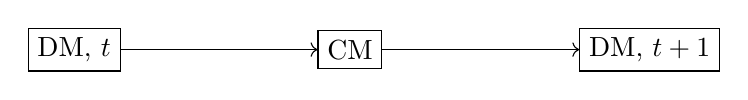
\begin{tikzpicture}[node distance=2.5cm]
        \node[draw, rectangle] (dm1) {DM, $t$};
        \node[draw, rectangle, right=of dm1] (cm) {CM};
        \node[draw, rectangle, right=of cm] (dm2) {DM, $t+1$};
        \draw[->] (dm1) -- (cm);
        \draw[->] (cm) -- (dm2);
    \end{tikzpicture}
    \end{center}
    \vspace{3mm}
    There are two nonstorable consumption goods: $x_t$ is produced and consumed in the CM; $y_t$ is produced and consumed in the DM. Households can convert labour time into goods one-for-one in the CM.
\end{frame}

\begin{frame}{Rocheteau and Wright}
    The utility of a household is
    \[
        \mathbb{E}_0 \sum_{t=0}^\infty \beta^t \mathcal{U}(y_t, x_t, h_t)
    \]
    Where $\beta \in (0, 1)$. Let $\mathcal{U}(y_t, x_t, h_t) = u(y_t) + U(x_t) - h_t$, where $u(y_t)$ and $U(x_t)$ are twice continuously differentiable, strictly increasing, and concave.
\end{frame}

\begin{frame}{Rocheteau and Wright}
    To participate in the DM at $t$, firms must invest $k^f > 0$ units of the CM good at $t-1$. This allows it to generate at $t$ any amount $y \in [0,1]$ of the DM good, plus $x = f(1 - y)$ of the CM goods, where $f$ is twice continuously differentiable, strictly increasing, and concave, $f'(0) = \infty$ and $f'(1) = 0$. This makes $c(y) \equiv f(1) - f(1-y)$ the opportunity cost of selling $y$ in the DM, where $c(0) = 0$, $c'(0) = 0$ and $c'(1) = \infty$.

    Assume $k^f > \beta f(1)$, so it is not profitable to produce only CM goods. One can think of firms as issuing equity to pay for the investment $k^f$: each share issued in the CM at $t-1$ at a normalised price of 1 entitles its holder to a fraction $1/k^f$ of profit at $t$.
\end{frame}

\begin{frame}{Rocheteau and Wright}
    Assume portfolios of households are fully diversified, and denote by $R_t$ the expected return. In addition to equity in these firms, there is another asset, in fixed supply $A > 0$, that one can think of as a standard Lucas tree, yielding $\kappa > 0$ units of $x$ each period in the CM. Let $q$ be the CM price of this asset in terms of $x$.
\end{frame}

\begin{frame}{Rocheteau and Wright}
    The DM involves bilateral random matching. The matching probabilities for households and firms are $\alpha(n)$ and $\alpha(n)/n$ respectively, where $n$ is the measure of participating firms. The properties of the matching probabilities are, $\alpha'(n) > 0$, $\alpha''(n) < 0$, $\alpha(n) \le \min\{1, n\}$, $\alpha(0) = 0$, $\alpha'(0) = 1$ and $\alpha(\infty) = 1$.
\end{frame}

\begin{frame}{Rocheteau and Wright}
    Let $W_t(a, s, d)$ be a household's value function in the CM at $t$ with $a$ units of the liquid asset, $s$ illiquid shares in firms, and debt $d$ from the previous DM, in units of $x$. Similarly, let $V_t(a, s)$ be their value function in the DM at $t$. Then we have
    \[
        W_t(a_t, s_t, d_t) = \max_{x_t, h_t, a_{t+1}, s_{t+1}} \{U(x_t) - h_t + \beta V_{t+1}(a_{t+1}, s_{t+1})\}
    \]
    Subject to
    \[
        x_t + d_t + q_t(a_{t+1} - a_t) + s_{t+1} = h_t + \kappa a_t + R_t s_t
    \]
    Where $q_t$ is the price of the liquid asset and $R_t$ the gross return on shares.
\end{frame}

\begin{frame}{Rocheteau and Wright}
    We can substitute the budget constraint in for $h_t$ and we obtain
    \begin{align*}
        W_t(a_t, s_t, d_t) &= (q_t + \kappa) a_t + R_t s_t - d_t + \max_{x_t} \{U(x_t) - x_t\} \\
        &\quad + \max_{a_{t+1}, s_{t+1}} \{-q a_{t+1} - s_{t+1} + \beta V_{t+1}(a_{t+1}, s_{t+1})\} \\
        &= (q_t + \kappa) a_t + R_t s_t - d_t + W_t(0, 0, 0)
    \end{align*}
    Notice that since $h_t$ is linear, it immediately implies $(a_{t+1}, s_{t+1})$ is independent of $(a_t, s_t, d_t)$, which means we do not have to track the distribution of assets across agents in the DM as a state variable.
\end{frame}

\begin{frame}{Rocheteau and Wright}
    Moving to the DM, in any meeting the firms gives the household output $y$ in exchange for $\tau_a$ liquid assets, $\tau_s$ stocks, and a promise (debt) of $d$ payable in the next CM. To determine the terms of trade, we use Kalai proportional bargaining solution with $\theta \in [0, 1]$ denoting the household's share, (we can also use generalised Nash bargaining as well, but for algebraic simplicity we will use Kalai's proportional bargaining):
    \[
        (y_t, \tau_{a,t}, \tau_{s,t}, d_t) = \arg \max_{y, \tau_a, \tau_s, d} \{u(y) + W_t(a - \tau_a, s - \tau_s, d) - W_t(a, s, 0)\}
    \]
    Subject to
    \[
        u(y) + W_t(a - \tau_a, s - \tau_s, d) - W_t(a, s, 0) = \frac{\theta}{1-\theta}[f(1 - y) + (q_t + \kappa)\tau_a + R_t \tau_s + d - f(1)]
    \]
    We can simplify this problem.
\end{frame}

\begin{frame}{Rocheteau and Wright}
    Simplifying the CM component of the household surplus
    \begin{align*}
        W_t(a - \tau_a, s - \tau_s, d) - W_t(a, s, 0) &= (q_t + \kappa)(a - \tau_a) + R_t(s - \tau_s) - d + W_t(0,0,0) \\
        &\quad - [(q_t + \kappa) a + R_t s + W_t(0,0,0)] \\
        &= -(q_t + \kappa) \tau_a - R_t \tau_s - d
    \end{align*}
\end{frame}

\begin{frame}{Rocheteau and Wright}
    Simplifying the budget constraint we note that $c(y) = f(1) - f(1-y)$. Therefore we get
    \[
        u(y) - (q_t - \kappa) \tau_a - R_t \tau_s - d = \frac{\theta}{1-\theta} [-c(y) + (q_t + \kappa) \tau_a + R_t \tau_s + d]
    \]
    Rearranging we get
    \[
        (q_t + \kappa) \tau_a + R_t \tau_s + d = (1-\theta) u(y) + \theta c(y)
    \]
    We must also include the following constraints on asset transfers to the bargaining problem: $\tau_a \le a$, and $\tau_s \le \min(s, \bar \tau_s)$, where $\bar \tau_s$ is an upper bound that arises because of the recognisability problem, if stocks are freely counterfeitable and not verifiable then $\bar \tau_s = 0$.
\end{frame}

\begin{frame}{Rocheteau and Wright}
    Therefore the Kalai proportional bargaining problem becomes
    \[
        (y_t, \tau_{a,t}, \tau_{s,t}, d_t) = \arg \max_{y, \tau_a, \tau_s, d} \{u(y) - (q_t + \kappa)\tau_a - R_t \tau_s - d\}
    \]
    Subject to
    \[
        (q_t + \kappa)\tau_a + R_t \tau_s + d = (1-\theta) u(y) + \theta c(y), \quad \tau_a \le a, \quad \tau_s \le \min(s, \bar \tau_s)
    \]
\end{frame}

\begin{frame}{Rocheteau and Wright}
    \textbf{Perfect Credit}

    We can show that $y_t = y^*$ and as a result
    \[
        (q_t + \kappa)\tau_{a,t} + R_t \tau_{s,t} + d_t = (1-\theta) u(y^*) + \theta c(y^*)
    \]
    Thus we get efficient production $y_t = y^*$ in every DM meeting. Moreover, the exact form of payment --- in terms of $\tau_{a,t}, \tau_{s,t}$ or $d_t$ --- is irrelevant as long as the total payment has CM value $(1-\theta)u(y^*) + \theta c(y^*)$. Hence, we can impose without loss of generality that DM trade is conducted exclusively with debt, and the liquidity or illiquidity of assets is irrelevant for consumption or welfare.
\end{frame}

\begin{frame}{Rocheteau and Wright}
    Now moving to the DM value function. Given the linearity of $W_t$ and the bargaining solution
    \begin{align*}
        V_t(a, s) &= \alpha(n_t)[u(y^*) + W_t(a, s, d)] + [1 - \alpha(n_t)] W_t(a, s, 0) \\
        &= \alpha(n_t) \theta [u(y^*) - c(y^*)] + (q_t + \kappa) a + R_t s + W_t(0, 0, 0)
    \end{align*}
    We can substitute this into the CM value function to find the objective function to solve for the asset price.
\end{frame}

\begin{frame}{Rocheteau and Wright}
    Substituting the DM value function into the CM value function we get
    \begin{align*}
        W_t(a_t, s_t, d_t) &= (q_t + \kappa) a_t + R_t s_t - d_t + \max_{x_t}\{U(x_t) - x_t\} \\
        &\quad + \max_{a_{t+1}, s_{t+1}} \Big\{ -q_t a_{t+1} - s_{t+1} + \beta \big( \alpha(n_{t+1}) \theta [u(y^*) - c(y^*)] \\
        &\qquad\qquad + (q_{t+1} + \kappa) a_{t+1} + R_{t+1} s_{t+1} + W_{t+1}(0,0,0) \big) \Big\}
    \end{align*}
\end{frame}

\begin{frame}{Rocheteau and Wright}
    Focusing on the objective for $\{a_{t+1}, s_{t+1}\}$, rolling one period back and removing all variables and functions that do not depend on $a_t$ or $s_t$, we get
    \[
        \max_{a_t, s_t} \{-q_{t-1} a_t - s_t + \beta (q_t + \kappa) a_t + \beta R_t s_t\}
    \]
    Rearranging we get
    \[
        \max_{a, s}\{-[q_{t-1} - \beta(q_t + \kappa)] a - [1 - \beta R_t] s\}
    \]
    Splitting this optimisation
    \[
        \max_a \{-[q_{t-1} - \beta(q_t + \kappa)] a\} + \max_s \{(-1 + \beta R_t) s\}
    \]
\end{frame}

\begin{frame}{Rocheteau and Wright}
    Taking the first order condition with respect to $a$, we get
    \[
        q_{t-1} = \beta (q_t + \kappa)
    \]
    Noting that $R_t = \beta^{-1}$, where $R_t = (1 + r_t)$, we get
    \[
        \beta^{-1} = \frac{q_t + \kappa}{q_{t-1}} \implies q_{t-1} = \frac{q_t + \kappa}{1 + r}
    \]
    Given nonnegativity $q_t \ge 0$, together with the transversality condition $\lim_{t \to \infty} \beta^t q_t = 0$, the only admissible solution to this difference equation is $q_t = q^*$, where
    \[
        q^* = \frac{\kappa}{r}
    \]
    Which is the fundamental price of the asset.
\end{frame}

\begin{frame}{Rocheteau and Wright}
    It remains to determine entry. The expected value of a firm in the DM at $t$ is
    \[
        \Pi_t = \frac{\alpha(n_t)}{n_t}[f(1 - y^*)] + \left[1 - \frac{\alpha(n_t)}{n_t}\right] f(1)
    \]
    Which says that with probability $\alpha(n_t)/n_t$ the firm meets a household in the DM and sells $y^*$ for a promise of $d_t = (1 - \theta) u(y^*) + \theta c(y^*)$ in the next CM, and then sells $f(1 - y_t)$ in the CM. With complementary probability $1 - \frac{\alpha(n_t)}{n_t}$, the firm is unmatched in the DM and sells $f(1)$ in the CM.
\end{frame}

\begin{frame}{Rocheteau and Wright}
    Firms participate in the DM as long as $\Pi_t \le R_t k^f$. Using $\beta R_t = 1$, the measure of entrants $n_t$ solves
    \[
        \frac{\alpha(n_t)}{n_t}(1 - \theta)[u(y^*) - c(y^*)] \le k, \quad = \text{ if } n_t > 0
    \]
    Where $k \equiv \frac{k^f}{\beta} - f(1)$, thus we can write
    \[
        n_t = \psi^{-1}\left( \min \left\{ \frac{k}{(1-\theta)[u(y) - c(y)]}, 1 \right\} \right)
    \]
    Where $\psi(n_t) = \alpha(n_t)/n_t$.
\end{frame}

\begin{frame}{Rocheteau and Wright}
    With perfect credit the equilibrium is efficient iff
    \[
        1 - \theta = \frac{n^* \alpha'(n^*)}{\alpha(n^*)}
    \]
    Where $n^*$ solves $\alpha(n)[u(y^*) - c(y^*)] = k$.
\end{frame}

\section{Imperfect Credit}

\begin{frame}{Rocheteau and Wright}
    \textbf{Imperfect Credit}

    Now consider an economy where households cannot commit to repay debt, which means $d_t = 0$. In this economy, the liquidity of assets can be critical. We continue to assume that shares in firms are not recognisable, so $\bar \tau_s = 0$. The CM value function of the household is still given by the same equation, but since credit is not feasible we omit the third argument of $W_t$, i.e.
    \begin{align*}
        W_t(a_t, s_t) &= (q_t + \kappa) a_t + R_t s_t + \max_{x_t}\{U(x_t) - x_t\} \\
        &\quad + \max_{a_{t+1}, s_{t+1}}\{-q_t a_{t+1} - s_{t+1} + \beta V_{t+1}(a_{t+1}, s_{t+1})\}
    \end{align*}
\end{frame}

\begin{frame}{Rocheteau and Wright}
    Moving now to the Kalai proportional bargaining problem in this case, again remembering $d_t = \bar \tau_s = 0$, we can write
    \[
        (y_t, \tau_{a,t}) = \arg \max_{y, \tau_a} \{u(y) - (q_t + \kappa) \tau_a\}
    \]
    Subject to
    \[
        (q_t + \kappa) \tau_a = (1 - \theta) u(y) + \theta c(y), \quad \text{and} \quad \tau_a \le a
    \]
\end{frame}

\begin{frame}{Rocheteau and Wright}
    Simplifying the Kalai proportional bargaining problem, we get
    \[
        y_t = \arg \max_y \{\theta [u(y) - c(y)]\}
    \]
    Subject to
    \[
        \tau_{a,t} = \frac{(1-\theta) u(y) + \theta c(y)}{q_t + \kappa} \le a
    \]
    If $\tau_{a,t} \le a$ does not bind then $y_t = y^*$ and
    \[
        \tau_{a,t} = \frac{(1-\theta) u(y^*) + \theta c(y^*)}{q_t + \kappa}
    \]
    If it does bind, the $y_t$ is the solution to
    \[
        (q_t + \kappa) a = \omega(y_t)
    \]
    Where $\omega(y_t) = \theta c(y_t) + (1-\theta) u(y_t)$. The important point to note about this solution is that $y_t$ is a function of a household's liquid wealth.
\end{frame}

\begin{frame}{Rocheteau and Wright}
    The DM value function is the same as before, noting this time that $y$ is a function of $a$
    \[
        V_t(a, s) = \alpha(n_t) \theta \{u[y((q_t + \kappa) a)] - c[y((q_t + \kappa) a)]\} + (q_t + \kappa) a + R_t s + W_t(0,0)
    \]
    Substituting this value function into the CM value function, we get the same optimisation as before
    \[
        \max_a \{-q_{t-1} a + \beta \alpha(n_t) \theta (u[y((q_t + \kappa) a)] - c[y((q_t + \kappa) a)]) + \beta(q_t + \kappa) a\}
    \]
    Rearranging we get
    \[
        \max_a\left\{ -\left[\frac{q_{t-1}}{\beta} - (q_t + \kappa)\right] a + \alpha(n_t) \theta (u[y((q_t + \kappa) a)] - c[y((q_t + \kappa) a)])\right\}
    \]
\end{frame}

\begin{frame}{Rocheteau and Wright}
    Taking first-order conditions, we get
    \[
        \frac{q_{t-1}}{\beta} - (q_t + \kappa) = \alpha(n_t) \theta [u'(y) - c'(y)] y'(a)
    \]
    We have that
    \[
        (q_t + \kappa) a = \theta c(y) + (1 - \theta) u(y)
    \]
    Taking the first derivative
    \[
        q_t + \kappa = [\theta c'(y) + (1-\theta) u'(y)] y'(a) \implies y'(a) = \frac{q_t + \kappa}{\theta c'(y) + (1-\theta) u'(y)}
    \]
    Substituting this into the first order condition
    \[
        \frac{q_{t-1}}{\beta} - (q_t + \kappa) = (q_t + \kappa) \alpha(n_t) \theta \left[ \frac{u'(y) - c'(y)}{\theta c'(y) + (1-\theta) u'(y)}\right]
    \]
\end{frame}

\begin{frame}{Rocheteau and Wright}
    Rearranging, with imperfect credit, the price of the liquid asset satisfies the first order difference equation
    \[
        q_{t-1} = \Gamma(q_t) \equiv \frac{q_t + \kappa}{1 + r}\left\{ 1 + \alpha(n_t) \theta \left[ \frac{u'(y) - c'(y)}{\theta c'(y) + (1 - \theta) u'(y)}\right]\right\}
    \]
    Where
    \[
        y_t = \min\{y^*, \omega^{-1}[(q_t + \kappa) A]\}
    \]
    \[
        n_t = \psi^{-1}\left( \min \left\{ \frac{k}{(1-\theta)[u(y) - c(y)]}, 1\right\}\right)
    \]
    The price of the liquid asset at $t-1$ equals the discounted sum of the price plus dividend at $t$, multiplied by a liquidity factor. Any equilibrium $\{q_t\}_{t=0}^\infty$ must also satisfy $q_t \ge q^*$, since the price cannot be less than the fundamental price.
\end{frame}

\begin{frame}{Rocheteau and Wright}
    To analyse $q_{t-1} = \Gamma(q_t)$, we define two thresholds. The first is the price above which households have enough liquidity to buy $y^*$, given
    \[
        y_t = \min\{y^*, \omega^{-1}[(q_t + \kappa) A]\}
    \]
    Which becomes
    \[
        y^* = \omega^{-1}[(\bar q + \kappa) A]
    \]
    Rearranging, the threshold becomes
    \[
        \bar q = \frac{\omega(y^*)}{A} - \kappa
    \]
\end{frame}

\begin{frame}{Rocheteau and Wright}
    The second threshold is the price below which firms stop participation in the DM
    \begin{align*}
        \underline q &= \frac{\omega \left[ \Delta^{-1} \left(\frac{k}{1-\theta}\right)\right]}{A} - \kappa \quad \text{if } \frac{k}{1-\theta} \le u(y^*) - c(y^*) \\
        &= \infty
    \end{align*}
    Where $\Delta(y) = u(y) - c(y)$ for $y \in [0, y^*]$.
\end{frame}

\begin{frame}{Rocheteau and Wright}
    We claim $\Gamma(q_t)$ is linear whenever $q_t \notin (\underline q, \bar q)$, because $q_t < \underline q$ implies $n_t = 0$ and $q_t > \bar q$ implies $y_t = y^*$, and either case the asset has no liquidity value at the margin. In contrast, $q_t \in (\underline q, \bar q)$ exceeds the fundamental price because the asset facilitates DM trade. So the nonlinear part of $\Gamma(q_t)$ reflects the existence of a liquidity premium or bubble.
\end{frame}

\begin{frame}{Rocheteau and Wright}
    \centering
    % TODO: figure - phase diagram and price dynamics from Rocheteau-Wright (2013)
    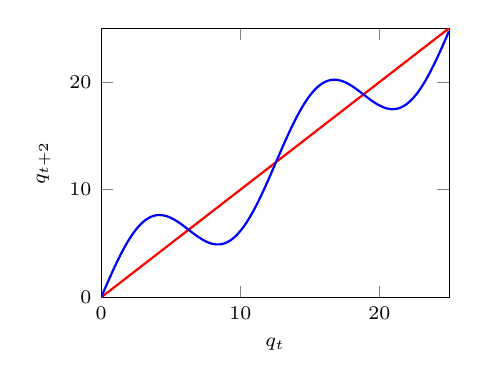
\begin{tikzpicture}
        \begin{axis}[
            width=6cm, height=5cm,
            xlabel={$q_t$}, ylabel={$q_{t+2}$},
            xmin=0, xmax=25, ymin=0, ymax=25,
            tick label style={font=\scriptsize}, label style={font=\scriptsize}
        ]
        \addplot[red, thick, domain=0:25] {x};
        \addplot[blue, thick, smooth, samples=80, domain=0:25] {x + 4*sin(deg(x/2))};
        \end{axis}
    \end{tikzpicture}
    \hspace{5mm}
    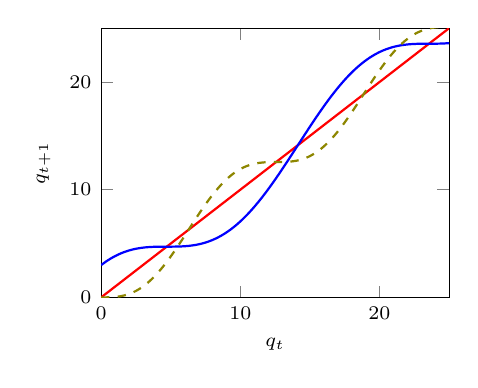
\begin{tikzpicture}
        \begin{axis}[
            width=6cm, height=5cm,
            xlabel={$q_t$}, ylabel={$q_{t+1}$},
            xmin=0, xmax=25, ymin=0, ymax=25,
            tick label style={font=\scriptsize}, label style={font=\scriptsize}
        ]
        \addplot[red, thick, domain=0:25] {x};
        \addplot[blue, thick, smooth, samples=80, domain=0:25] {x + 3*cos(deg(x/3))};
        \addplot[dashed, olive, thick, smooth, samples=80, domain=0:25] {x - 2*sin(deg(x/2))};
        \end{axis}
    \end{tikzpicture}
\end{frame}

\begin{frame}{Rocheteau and Wright}
    \centering
    % TODO: figure - asset price bubble trajectory
    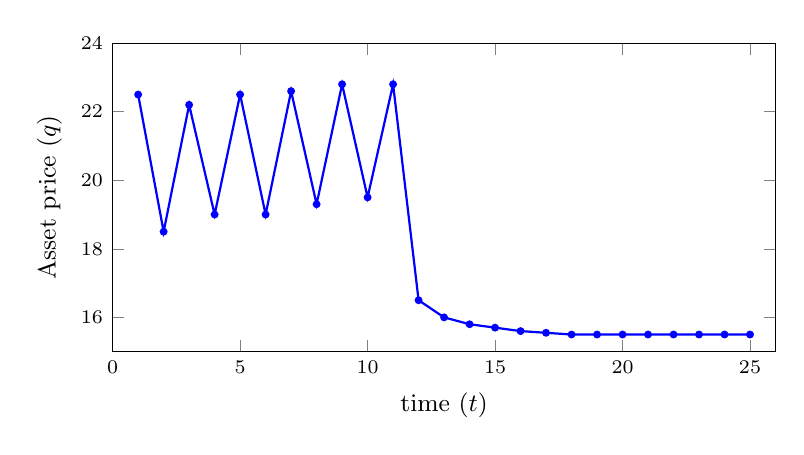
\begin{tikzpicture}
        \begin{axis}[
            width=10cm, height=5.5cm,
            xlabel={time ($t$)}, ylabel={Asset price ($q$)},
            xmin=0, xmax=26, ymin=15, ymax=24,
            tick label style={font=\scriptsize}, label style={font=\small}
        ]
        \addplot[blue, thick, mark=*, mark size=1pt] coordinates {
            (1,22.5) (2,18.5) (3,22.2) (4,19.0) (5,22.5) (6,19.0) (7,22.6) (8,19.3) (9,22.8) (10,19.5)
            (11,22.8) (12,16.5) (13,16.0) (14,15.8) (15,15.7) (16,15.6) (17,15.55) (18,15.5) (19,15.5)
            (20,15.5) (21,15.5) (22,15.5) (23,15.5) (24,15.5) (25,15.5)
        };
        \end{axis}
    \end{tikzpicture}
\end{frame}

\begin{frame}{Rocheteau and Wright}
    This bubble trajectory, with fluctuating asset prices followed by a crash, corresponds to the transition above. During the expansion phases, the return on the liquid asset is equal to the rate of time preference and households are not liquidity constrained, but the price cannot keep on increasing, or we would violate transversality.

    We have fluctuations around a high-price stationary equilibrium, but now we crash at some point toward a lower price equilibrium. The timing of the crash is indeterminate --- we can make it happen whenever we like. All agents in the model know the bubble will burst, and they know exactly when, in this perfect foresight equilibrium, but there is nothing they can do to either avoid it or profit from it.
\end{frame}

\begin{frame}[allowframebreaks]{References}
    \small
    \begin{thebibliography}{99}
        \bibitem[Rocheteau and Wright(2013)]{rw2013}
            Rocheteau, G.\ and R.\ Wright. Liquidity and asset-market dynamics. \textit{Journal of Monetary Economics}, 60(2):275--294, 2013.
    \end{thebibliography}
\end{frame}

\end{document}
